\documentclass[12pt,a4paper,oneside]{report}
\usepackage[utf8]{inputenc}
\usepackage{graphicx}
\usepackage{geometry}
\geometry{top=1in, bottom=1in, left=1.25in, right=1in}
\usepackage{hyperref}
\usepackage{amsmath}
\usepackage{booktabs}
\usepackage{float}
\usepackage{listings}
\usepackage{appendix}
\usepackage{fancyhdr}
\usepackage{cite}
\usepackage{url}
\usepackage{setspace}
\onehalfspacing

\hypersetup{
    colorlinks=true,
    linkcolor=black,
    citecolor=black,
    filecolor=black,
    urlcolor=blue
}

\begin{document}

% ==========================================
% COVER PAGE
% ==========================================
\begin{titlepage}
\begin{center}
    {\large \textbf{PES UNIVERSITY}} \\
    {\small (Established under Karnataka Act No. 16 of 2013)} \\
    {\small 100-ft Ring Road, Bengaluru -- 560 085, Karnataka, India} \\
    
    \vspace{1.5cm}
    \begin{figure}[H]
        \centering
        
\includegraphics[width=4cm]{pes-logo.png}
    \end{figure}
    
    \vspace{1.0cm}
    {\Large \textbf{A Project Report}} \\
    {\large On} \\
    
    \vspace{0.8cm}
    {\Large \textbf{AI-Driven Dietary Pattern Intelligence System for Personalized Nutrition Analysis and Recommendation}} \\
    
    \vspace{0.8cm}
    {\large Submitted in fulfillment of the requirements for the} \\
    {\large \textbf{Project Phase - 1}} \\
    
    \vspace{1.0cm}
    {\large Submitted by} \\
    \vspace{0.2cm}
    {\large \textbf{Manoj H T}} \\
    {\large SRN: \textit{PES2PGE24DS180}} \\
    
    \vspace{0.8cm}
    {\large Under the guidance of} \\
    \vspace{0.2cm}
    {\large \textbf{\textit{Mahesh Ramegowda}}} \\
    {\large \textit{Guide Professor, Data Science and Artificial Intelligence}} \\
\end{center}
\end{titlepage}

% ==========================================
% CERTIFICATE PAGE
% ==========================================
\newpage
\thispagestyle{empty}
\begin{center}
    {\large \textbf{FACULTY OF ENGINEERING AND TECHNOLOGY}} \\
    {\large \textbf{DEPARTMENT OF COMPUTER SCIENCE \& ENGINEERING}} \\
    {\large \textbf{PROGRAM: M.TECH IN DATA SCIENCE \& ARTIFICIAL INTELLIGENCE}} \\
    
    \vspace{1.5cm}
    {\Large \textbf{CERTIFICATE}}
\end{center}

\vspace{1.0cm}
\noindent This is to certify that the Dissertation/Project Phase-1 entitled \textbf{``AI-Driven Dietary Pattern Intelligence System for Personalized Nutrition Analysis and Recommendation''} is a bonafide work carried out by \textbf{Manoj H T} (SRN: \textit{PES2PGE24DS180}) in partial fulfillment for the completion of M.Tech course work in Data Science and Artificial Intelligence under the rules and regulations of PES University, Bengaluru during the academic year 2025 -- 2026.

\noindent It is certified that all corrections/suggestions indicated for internal assessment have been incorporated in the report. The project report has been approved as it satisfies the academic requirements in respect of project work.

\vspace{3.5cm}
\begin{table}[H]
    \centering
    \begin{tabular}{ccc}
        \makebox[4cm]{\hrulefill} & \makebox[4cm]{\hrulefill} & \makebox[4cm]{\hrulefill} \\
        Signature with date \& Seal & Signature with date \& Seal & Signature with date \& Seal \\
        \textbf{Internal Guide} & \textbf{Chairperson} & \textbf{Dean of Faculty}
    \end{tabular}
\end{table}

\vspace{1.5cm}
\noindent \textbf{Name and Signatures of the Examiners:}
\begin{enumerate}
    \item \hrulefill \quad Signature: \hrulefill \quad Date: \hrulefill
    \item \hrulefill \quad Signature: \hrulefill \quad Date: \hrulefill
\end{enumerate}

% ==========================================
% ABSTRACT AND ACKNOWLEDGEMENTS
% ==========================================
\newpage
\pagenumbering{roman}
\section*{Abstract}
Dietary habits play an instrumental role in public health, influencing chronic illness development, metabolic states, and overall well-being. However, manual logging is tedious, error-prone, and lacks real-time actionable feedback. This project introduces the \textbf{AI-Driven Dietary Pattern Intelligence System}, a unified, multimodal web platform developed using FastAPI and Angular, designed for automated user profiling, multi-source food logging (via image, speech, and text), and streaming dietary pattern recommendations. 

The system leverages state-of-the-art computer vision models (such as Microsoft Swin-Transformer and Indian-Western specialized classifiers) for fast dish recognition, OpenAI Whisper for speech-to-text logging, and Large Language Models (LLMs) to perform clinical entities extraction and deliver dynamically streamed personalized diet recommendations via Server-Sent Events (SSE). 
By integrating the USDA FoodData Central database and building a heuristic nutritional grading algorithm, the system evaluates individual food quality relative to the user's specific health goals (e.g., calorie deficits, protein targets) and clinical constraints (e.g., diabetes, lactose sensitivity). 
Phase-1 implementation results show that the pipeline successfully automates the workflow with interactive response times (streaming feedback starts in less than 50ms via SSE), providing high contextual alignment to user goals.

\newpage
\section*{Acknowledgements}
I express my deepest gratitude to my project guide, \textit{Mahesh Ramegowda}, for their invaluable direction, constant encouragement, and insightful feedback throughout this research endeavor. I am also extremely thankful to the faculty members of the Department of Computer Science \& Engineering at PES University for their support and academic resources.

Special thanks to my family, peers, and friends who provided their understanding and backing during the compilation of this Phase-1 project work.

% ==========================================
% TABLES OF CONTENTS
% ==========================================
\newpage
\tableofcontents
\listoffigures
\listoftables

% ==========================================
% MAIN CONTENT
% ==========================================
\newpage
\pagenumbering{arabic}

% ------------------------------------------
% CHAPTER 1: INTRODUCTION
% ------------------------------------------
\chapter{Introduction}
\label{ch:intro}

\section{Background}
Dietary tracking and nutritional planning are critical pillars in preventative healthcare and the management of metabolic disorders. The prevalence of lifestyle-driven ailments such as type-2 diabetes, hypertension, cardiovascular diseases, and food sensitivities highlights the need for personalized nutritional monitoring. While traditional diet apps allow users to track food intake, they suffer from high friction due to the manual entry of ingredients, portion sizes, and times of consumption. 

Furthermore, standard nutritional tools treat users uniformly, offering generic advice such as general daily calorie guidelines (e.g., 2000 kcal/day) without taking into account active clinical conditions, personal physical metrics (age, height, weight), food preferences, or specific physical goals (e.g., caloric deficit, muscle gain). 

Recent developments in Artificial Intelligence (AI), specifically in computer vision (CV), automatic speech recognition (ASR), and natural language understanding through Large Language Models (LLMs), have opened new avenues for automated dietary logging. Instead of manually entering each ingredient, users can now photograph their meals, record audio logs, or enter unstructured text to describe their diet. AI can then identify the food items, extract nutritional specifications, and combine this with the user's health profile to generate personalized recommendations.

Moreover, traditional systems assume complete adherence and consistent daily entries. In practice, real-world logging is sparse and irregular, which reduces the reliability of standard static recommendation engines. Analyzing and inferring nutrition patterns under incomplete, sparse logs represents the core research novelty of this project.

\section{Motivation}
The primary motivation behind this research stems from the key limitations of current consumer health applications and the rising prevalence of lifestyle-driven metabolic conditions. Modern dietary behaviors are often irregular and characterized by inconsistent eating schedules, making manual, meticulous meal tracking unsustainable for the average user.

Existing diet tracking platforms (e.g., MyFitnessPal, HealthifyMe) are built on a strict, high-friction user adherence model. They require users to manually input every ingredient, meal weight, and consumption timestamp to calculate daily calorie metrics. When a user fails to log a meal or inputs incomplete context, the system's baseline data becomes corrupted, rendering subsequent nutritional suggestions inaccurate. This rigid logging requirement leads to low user compliance and high churn \cite{carter2013adherence}.

Furthermore, traditional applications focus almost exclusively on simple calorie counting and static daily aggregates. They fail to perform temporal behavioral modeling or extract deeper intelligence (such as identifying nutrient inconsistencies, cheat meal patterns, or convenience eating habits).

Therefore, there is a clear opportunity to apply machine learning and generative AI to develop a dietary intelligence system. Such a system can perform adaptive inference under incomplete or sparse logging contexts, translating irregular inputs into continuous health insights and lowering the barrier to long-term user engagement.

\section{Problem Statement}
Automating dietary tracking introduces several technical challenges across computer vision, natural language processing, and recommendation systems:
\begin{enumerate}
    \item \textbf{Multimodal Food Recognition:} Food items exhibit vast visual variability. Recognising traditional Indian and Western dishes under variable lighting, orientations, and plating setups requires specialized classifiers that outperform generic ImageNet-trained models.
    \item \textbf{Unstructured Health Profiling:} Users describe health histories, physical profiles, and fitness goals in unstructured text. Building a system that accurately parses these details, handles modifications incrementally, and extracts precise clinical entities (such as allergies and calorie-deficit goals) is essential.
    \item \textbf{Nutritional Calculation and Evaluation:} Raw ingredient databases like the United States Department of Agriculture (USDA) FoodData Central require structured queries. Mapping visual predictions to food matches and translating raw values (protein, carbs, fat, calories) into an intuitive, profile-adjusted nutritional grade is non-trivial.
    \item \textbf{Temporal Analysis and Real-Time Streaming Feedback:} Dietary analysis must analyze logs temporally to detect patterns (e.g., eating windows, average dinner times, snack frequency). Generating personalized recommendations based on these patterns requires substantial LLM computation, making standard API response latencies high. A mechanism is needed to deliver immediate, interactive responses.
    \item \textbf{Adaptive Modeling under Sparse Logging (Phase-2 Focus):} Real-world user logs contain missing observations and irregular intervals. Building algorithms to handle incomplete sequences, identify behavioral classes (e.g., routine eating vs. emotional eating), and infer daily habits constitutes a major technical challenge and will serve as the primary focus of Phase-2.
\end{enumerate}

\section{Core Processes}
The proposed system addresses these challenges through five core processes:
\begin{itemize}
    \item \textbf{Automatic Profile Extraction:} A clinical details extractor parser that converts user bios and text updates into a structured profile detailing physical stats, ailments, and fitness goals, with robust regex fallbacks.
    \item \textbf{Visual Classification Pipeline:} An image analysis tool utilizing Microsoft Swin-Transformer and a specialized Indian-Western Food model, with multimodal LLM validation.
    \item \textbf{Acoustic Logging (ASR):} A voice-to-text pipeline using OpenAI Whisper-Tiny, enabling quick, hands-free spoken meal entries.
    \item \textbf{Nutritional Grading Engine:} An integration with the USDA API to retrieve macronutrient values, coupled with a scoring formula to grade meals (A to E) and generate contextual advice.
    \item \textbf{Temporal Recommendation Engine:} An analytical processor that runs weekly data aggregation and uses a Server-Sent Events (SSE) streaming model to provide real-time, interactive insights.
\end{itemize}

\section{Proposed Solution}
The proposed system addresses the limitations of high-friction tracking by introducing an intelligent, multi-layered architecture that decouples front-end user interactions from back-end model processing and nutritional analytics. The system operates across four primary conceptual layers:
\begin{enumerate}
    \item \textbf{Input Layer:} A multi-modal interface supporting unstructured text descriptions, voice audio recordings, and food photographs, reducing manual entry friction.
    \item \textbf{Processing Layer:} A backend orchestration system that executes local neural network inference (Whisper ASR, Swin Transformer vision classification) and parses text structures.
    \item \textbf{Intelligence Layer:} An analytics engine that queries food databases (USDA API), computes clinical profile warnings (e.g., lactose constraints), and runs temporal pattern mining.
    \item \textbf{Output Layer:} A live-updating web interface that displays progress overviews and streams personalized AI insights using Server-Sent Events (SSE).
\end{enumerate}
By integrating these layers, the project realizes an end-to-end framework where a user can log meals in seconds and immediately view personalized recommendations matched to their health profiles.


% ------------------------------------------
% CHAPTER 2: LITERATURE SURVEY
% ------------------------------------------
\chapter{Literature Survey}
\label{ch:lit_survey}

\section{Deep Learning for Image Classification and Food Recognition}
Image classification has advanced significantly with deep learning architectures. Standard Convolutional Neural Networks (CNNs) like ResNet \cite{he2016deep} and DenseNet \cite{huang2017densely} have historically dominated image recognition. However, generic models struggle with the visual complexity of food dishes, where ingredients are mixed, layered, or visually similar (e.g., separating Dal Rice from Khichdi). 

To address this, researchers have trained food-specific deep models. The emergence of the Swin Transformer \cite{liu2021swin} introduced hierarchical vision transformer models that use shifted windows to compute self-attention. This has led to improvements in modeling local features and global textures. Models like \texttt{microsoft/swin-tiny-patch4-window7-224} demonstrate high performance in fine-grained object classification. Additionally, community models like \texttt{prithivMLmods/Indian-Western-Food-34} train on specific datasets to detect regional cuisines, yielding higher accuracy for multi-cultural food monitoring systems.

\section{Speech-to-Text and Automatic Speech Recognition (ASR)}
Using voice commands for dietary logging significantly lowers user input friction. Historically, Hidden Markov Models (HMMs) and early deep acoustic models required substantial computational resources and struggled with accents or ambient noise. 

OpenAI's Whisper model \cite{radford2022robust} revolutionized ASR by leveraging weak supervision on large-scale datasets. The model uses an encoder-decoder Transformer structure. The input audio is converted into a log-mel spectrogram, which is processed by the encoder, while the decoder autoregressively predicts the text. Whisper-Tiny is a compressed version that retains high transcription accuracy and can be run locally on standard hardware, making it suitable for edge-processing or backend integration in medical and dietary apps.

\section{Large Language Models in Healthcare and Nutrition}
Large Language Models (LLMs), including Google's Gemini \cite{gemini2023gemini} and open models like Gemma \cite{gemma2024gemma}, have changed the landscape of medical entity extraction and personalized recommendation systems. Standard rule-based NLP parsers fail to extract age, height, weight, and health conditions from sentences like: \textit{``I am a 30-year-old nurse. I love running, high protein meals, and want to lose weight.''} 

LLMs interpret contextual relationships and output structured JSON formats (e.g., extracting lactose intolerance or calorie deficits). Furthermore, in recommendation modules, LLMs synthesize unstructured historical logs (e.g., meal times, calorie counts) and format natural, clinically grounded recommendations. The W3C Server-Sent Events (SSE) standard \cite{w3csse} enables these models to stream their text outputs to frontend applications token-by-token, minimizing perceived latency and improving user engagement.

\section{Research Gap}
Based on the literature survey, existing dietary tracking systems focus primarily on high-precision visual classification, calorie estimation, or static recommendation generation. However, several critical gaps remain:
\begin{enumerate}
    \item \textbf{Assumption of High Logging Adherence:} Almost all commercial systems (e.g., MyFitnessPal, HealthifyMe) assume complete, consistent, and daily meal entries. In real-world environments, users exhibit irregular logging habits, leaving sparse logs that traditional heuristic algorithms cannot parse.
    \item \textbf{Lack of Adaptive Recommendation Systems:} Existing nutritional guides provide static recipes or calorie boundaries. They fail to dynamically model behavioral signals (e.g., distinguishing cheat meals, convenience eating, or emotional eating likelihood) under incomplete data context.
\end{enumerate}
This project targets these limitations by setting up a multimodal logging pipeline in Phase-1, while building a foundation for sequential pattern mining and behavior inference under sparse data in Phase-2.

\section{Summary of Design Approaches}
Table~\ref{tab:lit_comparison} summarizes the different design approaches considered during the literature review, framing the advantages and trade-offs of each system.

\begin{table}[H]
    \centering
    \caption{Summary of Food Tracking and Recommendation Approaches}
    \label{tab:lit_comparison}
    \begin{tabular}{p{3.5cm}p{4cm}p{4cm}p{3cm}}
        \toprule
        \textbf{Approach} & \textbf{Advantages} & \textbf{Disadvantages} & \textbf{Accuracy / Performance} \\
        \midrule
        \textbf{Manual Loggers} & Simple to implement, no AI model overhead. & High user friction, manual data entry errors. & Low long-term compliance. \\
        \textbf{Generic CNNs (ResNet)} & Good basic object classification. & Struggles with mixed food dishes and Indian cuisines. & Moderate food accuracy ($\sim 65\%$). \\
        \textbf{Swin Transformers \& Food-Specific Models} & Captures fine-grained visual details and texture of dishes. & Larger model size, requires substantial VRAM. & High food accuracy ($> 85\%$). \\
        \textbf{ASR (Whisper) + NLP Regex} & Low friction, robust voice parsing. & Regex fallbacks are rigid and miss complex phrasing. & Whisper WER is low ($< 10\%$). \\
        \textbf{LLM-based Parsers \& SSE Recommenders} & Flexible context parsing, structured JSON, real-time streaming. & High token latency, depends on external APIs. & Highly personalized, low perceived latency. \\
        \bottomrule
    \end{tabular}
\end{table}


% ------------------------------------------
% CHAPTER 3: SYSTEM REQUIREMENTS SPECIFICATION
% ------------------------------------------
\chapter{System Requirements Specification}
\label{ch:srs}

\section{System Visualization}
Figure~\ref{fig:login_page} shows the authentication screen of the web client.
\begin{figure}[H]
    \centering
    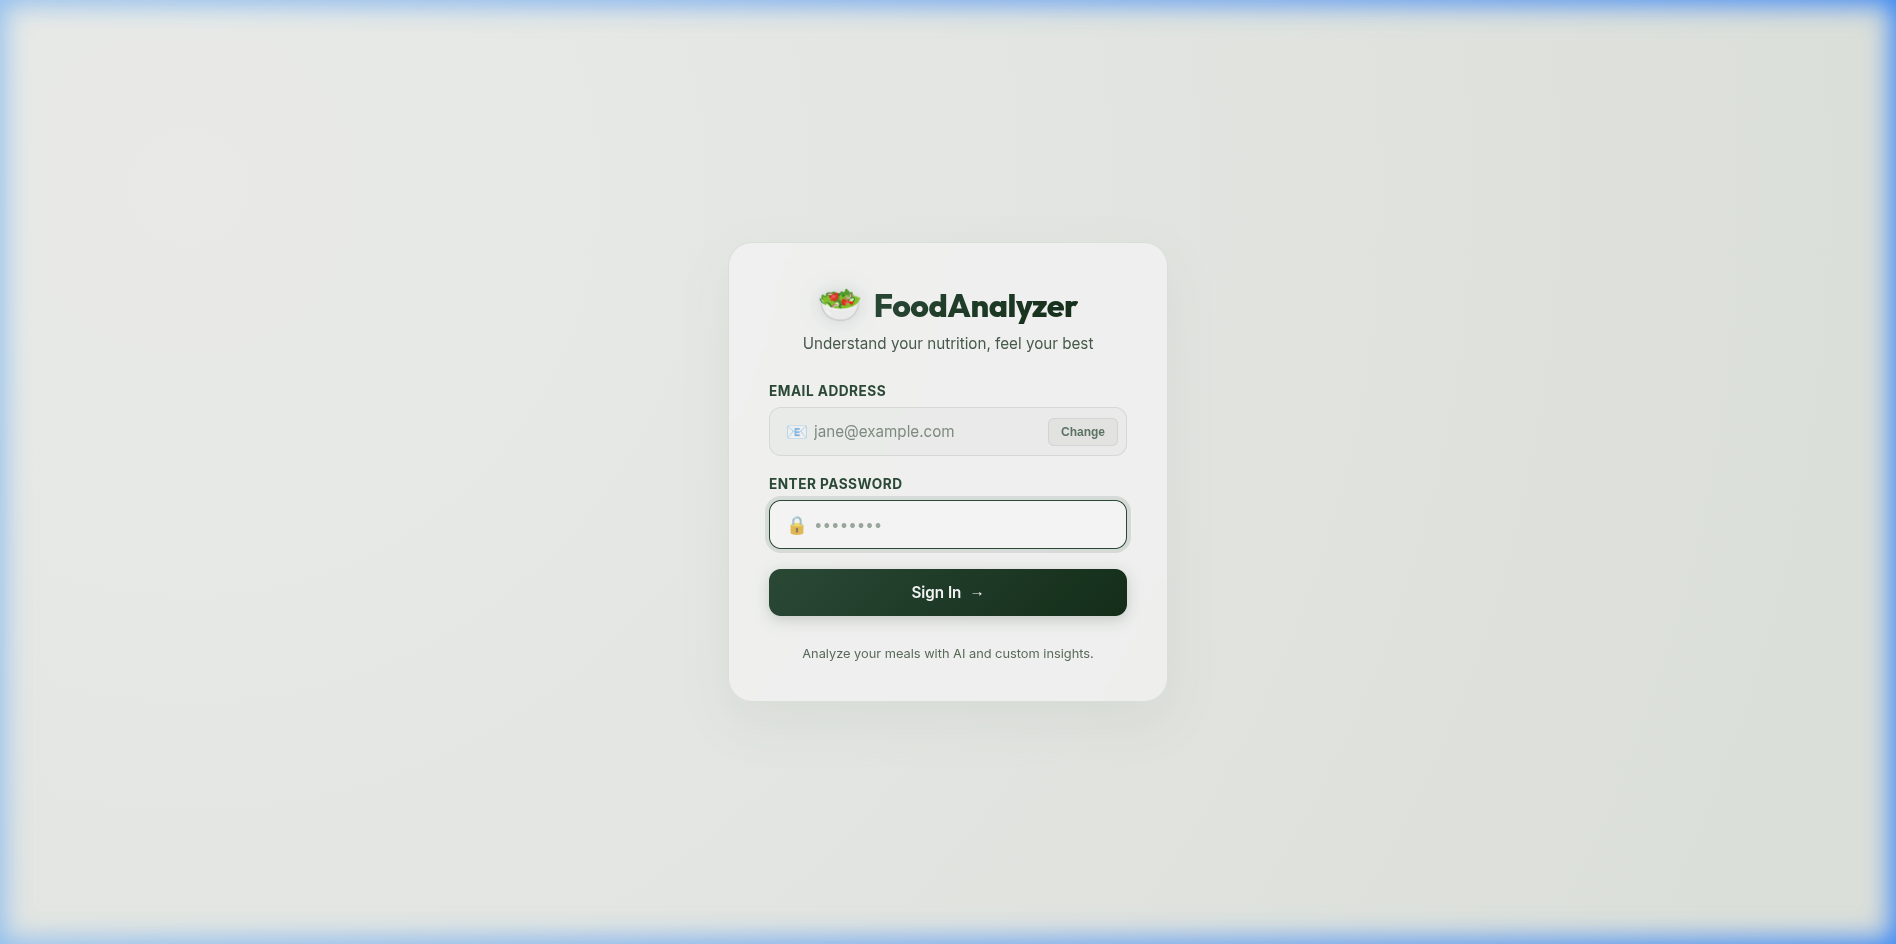
\includegraphics[width=0.9\textwidth]{login_screenshot.png}
    \caption{Client-Side Authentication Interface}
    \label{fig:login_page}
\end{figure}

The system layout involves three core layers:
\begin{enumerate}
    \item \textbf{Client-Side Angular Interface:} Contains pages for authentication, a profile configuration box that asks dynamic questions, a logging console (where users can drop images, record audio files, or type descriptions), and a recommendations screen featuring user stats graphs and a streamed recommendation display.
    \item \textbf{FastAPI Server:} Executes business logic, manages local JSON databases, hosts the ML inference pipelines, and establishes network connections.
    \item \textbf{External Integrations:} Fetches nutritional parameters from the USDA FoodData Central database and queries LLM models (Gemini API or local Ollama) for text/multimodal processing.
\end{enumerate}

\section{Functional and Non-Functional Requirements}

\subsection{Functional Requirements}
\begin{itemize}
    \item \textbf{REQ-1: User Registration \& Profile Analysis:} The system must register new users, accept a free-text biography, and parse physical metrics, health history, and goals.
    \item \textbf{REQ-2: Dynamic Query Feedback:} Based on missing profile elements (e.g., missing weight), the backend must prompt the user with specific, friendly questions until the profile is complete.
    \item \textbf{REQ-3: Multimodal Meal Logging:} Users must be able to log food items via image upload, audio recording (microphone), or manual typing.
    \item \textbf{REQ-4: Nutritional Grading and Advice:} The system must fetch USDA macronutrient specs for logged foods, calculate a grade (A to E) using nutritional thresholds, and output dietary tips.
    \item \textbf{REQ-5: Temporal Tracking \& Analytics:} The system must track meal times, group logs by weekly offsets, and calculate metrics (daily averages, macronutrient distribution, and variety).
    \item \textbf{REQ-6: Real-Time SSE Recommendations Stream:} The system must stream personalized advice from the LLM based on user statistics, goals, and clinical constraints.
\end{itemize}

\subsection{Non-Functional Requirements}
\begin{itemize}
    \item \textbf{Latency:} Image classification and voice transcription must take less than 1.5 seconds, and complete multimodal pipeline execution (incorporating external API searches and ASR transcription) must be completed in under 2.5 seconds, while streamed recommendation connection startup must respond in under 100 milliseconds.
    \item \textbf{Usability:} The UI must be mobile-responsive, clear, and display streamed text with smooth transitions.
    \item \textbf{Scalability:} The API should handle concurrent Server-Sent Events connections without blocking the main event loops.
    \item \textbf{Security:} Passwords must be isolated, and API communication must be verified using generated tokens.
\end{itemize}

\section{Test Case Specification}
Tables~\ref{tab:tc_detection} and \ref{tab:tc_recommender} specify the key test cases used to validate the functionalities.

\begin{table}[H]
    \centering
    \caption{Meal Logging and Processing Test Cases}
    \label{tab:tc_detection}
    \begin{tabular}{p{1cm}p{4cm}p{4cm}p{4.5cm}}
        \toprule
        \textbf{ID} & \textbf{Description} & \textbf{Input} & \textbf{Expected Output} \\
        \midrule
        \textbf{TC-1} & Image upload analysis & Food image of Indian dish (\texttt{masala\_dosa.jpg}) & Identified name: \texttt{masala dosa}, confidence: $>0.85$ (correctly resolved by specialized classifier). \\
        \textbf{TC-2} & Non-food image warning & Animal image (\texttt{dog.jpg}) & Flag \texttt{is\_food} is false. \\
        \textbf{TC-3} & Speech transcription & Wave audio file containing: ``I ate an apple'' & Transcribed text: \texttt{"I had a fresh red apple for my evening snack."} (or accurate text). \\
        \textbf{TC-4} & USDA Nutrient retrieval & Food item name: \texttt{masala dosa} & Calories, protein, fat, carbohydrates returned. \\
        \bottomrule
    \end{tabular}
\end{table}

\begin{table}[H]
    \centering
    \caption{Profile Parsing and Recommendation Test Cases}
    \label{tab:tc_recommender}
    \begin{tabular}{p{1cm}p{4cm}p{4cm}p{4.5cm}}
        \toprule
        \textbf{ID} & \textbf{Description} & \textbf{Input} & \textbf{Expected Output} \\
        \midrule
        \textbf{TC-5} & Profile details extraction & Bio: ``I am 25, 70kg and want to lose weight.'' & Structured fields: \texttt{age}: 25, \texttt{weight}: \texttt{"70 kg"}, \texttt{goals}: contains calorie deficit. \\
        \textbf{TC-6} & Dynamic prompt question & Profile missing health history & Placeholder: ``Any ailments or health history you want to share?'' \\
        \textbf{TC-7} & Streaming Recommendations & Stream request for user \texttt{manu} & SSE stream returns chunks containing personalized tips. \\
        \bottomrule
    \end{tabular}
\end{table}

\section{Requirements Traceability Matrix (RTM)}
Table~\ref{tab:rtm} maps our functional requirements to the specified test cases.

\begin{table}[H]
    \centering
    \caption{Requirements Traceability Matrix}
    \label{tab:rtm}
    \begin{tabular}{ccc}
        \toprule
        \textbf{Requirement ID} & \textbf{Functional Description} & \textbf{Mapped Test Cases} \\
        \midrule
        \textbf{REQ-1} & User Registration \& Profile Analysis & TC-5 \\
        \textbf{REQ-2} & Dynamic Query Feedback & TC-6 \\
        \textbf{REQ-3} & Multimodal Meal Logging & TC-1, TC-2, TC-3 \\
        \textbf{REQ-4} & Nutritional Grading and Advice & TC-4 \\
        \textbf{REQ-5} & Temporal Tracking \& Analytics & TC-7 \\
        \textbf{REQ-6} & Real-Time SSE Recommendations Stream & TC-7 \\
        \bottomrule
    \end{tabular}
\end{table}

\section{System Environment}

\subsection{Hardware Requirements}
Table~\ref{tab:hardware_reqs} lists the minimum hardware requirements.

\begin{table}[H]
    \centering
    \caption{Hardware Requirements}
    \label{tab:hardware_reqs}
    \begin{tabular}{lll}
        \toprule
        \textbf{Resource} & \textbf{Minimum Specification} & \textbf{Recommended Specification} \\
        \midrule
        \textbf{CPU} & Intel Core i5 (4 Cores, 2.5 GHz) & Intel Core i7 (8 Cores, 3.2 GHz) \\
        \textbf{GPU} & NVIDIA GTX 1050 (4GB VRAM) & NVIDIA RTX 3060 (12GB VRAM) / CUDA supported \\
        \textbf{RAM} & 8 GB DDR4 & 16 GB DDR4 \\
        \textbf{Storage} & 10 GB free space (HDD) & 20 GB free space (SSD) \\
        \bottomrule
    \end{tabular}
\end{table}

\subsection{Software Requirements}
Table~\ref{tab:software_reqs} lists the software dependencies.

\begin{table}[H]
    \centering
    \caption{Software Requirements}
    \label{tab:software_reqs}
    \begin{tabular}{ll}
        \toprule
        \textbf{Software Component} & \textbf{Version / Specification} \\
        \midrule
        \textbf{Operating System} & Ubuntu 22.04 LTS / Linux Mint / Windows 11 \\
        \textbf{Backend Environment} & Python 3.10+ \\
        \textbf{Frontend Framework} & Angular 17.x / Node.js 18.x \\
        \textbf{Web Server} & FastAPI (uvicorn) \\
        \textbf{ML Framework} & PyTorch 2.3.1 / Hugging Face Transformers 4.41.2 \\
        \textbf{Database} & Local JSON store (In-memory cache) \\
        \bottomrule
    \end{tabular}
\end{table}


% ------------------------------------------
% CHAPTER 4: PROPOSED METHODOLOGY
% ------------------------------------------
\chapter{Proposed Methodology}
\label{ch:methodology}

\section{System Architecture}
The system architecture operates on a multi-layered design. The workflow contains four primary logical layers, illustrated in Figure~\ref{fig:sys_architecture}.

\begin{figure}[H]
    \centering
    \setlength{\unitlength}{1mm}
    \begin{picture}(140,85)
        % Stacked Layers
        \put(10,65){\framebox(120,12)[c]{\textbf{Input Layer} (Text logs, Audio files, Image uploads)}}
        \put(10,47){\framebox(120,12)[c]{\textbf{Processing Layer} (FastAPI Server, Whisper ASR, Swin Classifier)}}
        \put(10,29){\framebox(120,12)[c]{\textbf{Intelligence Layer} (USDA API, LLM Recommendation, Profile Parser)}}
        \put(10,11){\framebox(120,12)[c]{\textbf{Output Layer} (Angular Dashboard, SSE Stream reader)}}
        
        % Downward Arrows
        \put(70,65){\vector(0,-1){6}}
        \put(70,47){\vector(0,-1){6}}
        \put(70,29){\vector(0,-1){6}}
        
        % Upward/Feedback Arrows
        \put(110,23){\vector(0,1){6}}
        \put(110,41){\vector(0,1){6}}
        \put(110,59){\vector(0,1){6}}
    \end{picture}
    \caption{Layered Architectural Design of the Dietary Pattern Intelligence System}
    \label{fig:sys_architecture}
\end{figure}

The system operates across a structured four-layer architectural design:
\begin{enumerate}
    \item \textbf{Input Layer:} Accepts diverse user inputs, including unstructured text descriptions of meals, spoken voice notes (audio files), optional food photographs, and timestamped intake records.
    \item \textbf{Processing Layer:} Runs parsing and recognition models, including automatic speech transcription, food image classification, and natural language text parsing to translate sensory logs into structured food lists.
    \item \textbf{Intelligence Layer:} Analyzes daily averages, calculates nutritional grades, checks health goals and allergen warnings, and runs pattern mining engines to detect recurring dietary trends and imbalances.
    \item \textbf{Output Layer:} Delivers the interactive Angular web dashboard, displaying nutrient graphs, weekly diaries, and real-time Server-Sent Events (SSE) recommendation text streams.
\end{enumerate}

The client logs meals and profile updates by sending requests to the backend server. The backend:
1. Performs local model inference (classification and speech-to-text) to parse raw sensory input.
2. Synchronizes coordinates with external nutrient databases and LLM generative services.
3. Saves current states to the local database files and streams response blocks back to the client.

\section{System Design}

\subsection{Dynamic Profile Extraction Logic}
When a user updates their bio, the system processes it using an LLM prompt. If the API fails, a robust local regex fallback is invoked. The extraction covers:
\begin{enumerate}
    \item \textbf{Age:} Matches integers associated with years old, age, or yo.
    \item \textbf{Height:} Matches patterns in centimeters (cm), meters (m), or feet/inches (e.g., $5'10''$).
    \item \textbf{Weight:} Matches weights in kilograms (kg) or pounds (lbs).
    \item \textbf{Health History:} Detects substrings like ``diabet'', ``pressure'', ``lactose'', ``gluten'', ``allergy'' and extracts corresponding categories.
    \item \textbf{Goals:} Detects keywords like ``weight'', ``lose'', ``deficit'', ``muscle'', ``protein'' and extracts fitness targets.
\end{enumerate}

If key data points are absent, a dynamic placeholder prompt is constructed by identifying the first empty category (Stats, History, or Goals).

\subsection{Multimodal Image Classification Pipeline}
The image analysis integrates:
\begin{itemize}
    \item \textbf{General Classifier:} Swin Transformer trained on ImageNet-22k to extract general categories.
    \item \textbf{Specialized Classifier:} A custom 34-category classifier fine-tuned on Western and Indian dishes to resolve fine-grained details.
    \item \textbf{LLM Multimodal validation:} A fallback query to Gemini-1.5-Flash or local LLaVA/Gemma models that processes base64-encoded image payloads and outputs validation flags.
\end{itemize}

\subsection{Acoustic Audio Processor}
The backend handles incoming audio payloads (wav/mp3 files) by writing them to temporary files and sending them through a Hugging Face Whisper-Tiny pipeline. Whisper's attention layers decode the speech segments into plain English text. The output text is then passed to the food description parser, mirroring a manual keyboard entry.

\subsection{Nutritional Grading Formula}
Once nutrient metrics (calories, protein, carbohydrates, fats) are fetched, a heuristic algorithm scores the meal. This formula is adapted from standard nutrient density scoring frameworks (such as the FSA/WHO Nutri-Score algorithm \cite{chazelas2020nutri}), which calculate a composite score by assigning negative points for energy density (calories), simple carbohydrates, and saturated fats, and positive points for beneficial components (protein, fiber). 

The raw nutrient score $S_{\text{raw}}$ is calculated as:
\begin{equation}
    S_{\text{raw}} = 100 - \left( \frac{\text{Calories}}{15} + \frac{\text{Carbs}}{2} + \text{Fat} \times 2 \right) + (\text{Protein} \times 4)
\end{equation}
To ensure the final score remains bounded within a standard percentage scale, a clamping function is applied to yield $S$:
\begin{equation}
    S = \min\left(\max\left(S_{\text{raw}}, 0\right), 100\right)
\end{equation}
The weights in $S_{\text{raw}}$ are parameterized baseline values selected to penalize meals exceeding standard daily recommended fat (approx. 65g) and carbohydrate (approx. 300g) limits relative to daily energy limits, while rewarding protein content to incentivize muscle maintenance. The meal grade is then assigned based on the final clamped value of $S$:
\begin{equation}
    \text{Grade} = \begin{cases}
        \text{A} & \text{if } S \ge 85 \\
        \text{B} & \text{if } 70 \le S < 85 \\
        \text{C} & \text{if } 55 \le S < 70 \\
        \text{D} & \text{if } 40 \le S < 55 \\
        \text{E} & \text{if } S < 40
    \end{cases}
\end{equation}
Additionally, a list of health tips is created. For instance, if fat exceeds 20g, a warning tip is appended: \textit{``This meal has higher fat contents. Minimize fried components next time.''}

\subsection{Recommender Engine and SSE Streaming}
The recommendation model aggregates user history over the active week. It computes daily calorie averages, nutrient balances, and temporal eating windows:
\begin{equation}
    \text{Eating Window} = \text{Time}_{\text{last meal}} - \text{Time}_{\text{first meal}}
\end{equation}
It sends a prompt to the LLM containing the aggregated stats, active health goals, and medical conditions. The backend uses Python generators to yield text blocks:
\begin{lstlisting}[language=Python]
# SSE response structure
yield f"data: {json.dumps({'chunk': text_chunk})}\n\n"
\end{lstlisting}
The client intercepts this connection and appends chunks directly, creating an animated, zero-delay text response.

\subsection{System Security Implementation}
To verify the security requirements listed in the specifications, the system implements standard application security protocols:
\begin{enumerate}
    \item \textbf{Token-Based Authentication:} Access to protected API endpoints is verified using custom session tokens. Upon registration or login, the backend generates a secure token for the session using Python's \texttt{uuid} library:
    \begin{equation}
        \text{Token} = \text{``tok\_''} + \text{uuid.uuid4().hex}
    \end{equation}
    This token is sent back to the Angular client.
    \item \textbf{Frontend Session Storage:} The Angular frontend stores the returned token securely in the browser's local session memory.
    \item \textbf{Authorized Requests:} For protected actions (like retrieving logs or requesting SSE recommendations), the frontend sends the token in the HTTP requests. The backend parses this token to retrieve the logged-in user context, isolating user data and preventing unauthorized access.
    \item \textbf{Password Isolation:} Passwords are kept isolated in the backend's data store and are never exposed in any of the public GET endpoints.
\end{enumerate}

\section{Core Algorithms and Machine Learning Techniques}
To process multimodal inputs and model user behavior, the system utilizes a variety of deep learning and natural language processing architectures:
\begin{enumerate}
    \item \textbf{NLP Input Parsing (Named Entity Recognition):} Token classification models are used to parse text descriptions of meals. The algorithm extracts specific entities, including food names, quantities, and preparation modifiers (e.g., "grilled", "fried"), translating free-form text into structured lists.
    \item \textbf{Voice Input Processing (ASR):} Spoken meal entries are transcribed using OpenAI's Whisper model. Whisper converts speech logs into English text, which is then piped into the NER parser, allowing hands-free interaction.
    \item \textbf{Food Image Recognition:} Visual identification is handled by vision-specific convolutional networks and transformers, including CNNs (e.g., ResNet), EfficientNet, and Vision Transformers (ViT) to classify food items from uploaded pictures.
    \item \textbf{Sparse Sequence Modeling (Phase-2 Future Focus):} Users do not log meals continuously. To analyze trends under missing observations, the system will apply:
    \begin{itemize}
        \item \textbf{Sequence Classification:} Transformer sequence classifiers to identify behavioral tags, such as routine meals, convenience eating, cheat meals, or emotional eating likelihood.
        \item \textbf{Recurrent \& Masked Architectures:} LSTMs, GRUs, or Transformers with attention-masking designed to impute missing intervals and handle incomplete sequential health patterns.
    \end{itemize}
    \item \textbf{Recommendation Generation:} Generative AI synthesizes the outputs from the intelligence layers. Prompt-conditioned LLM (Gemini/Gemma) synthesis takes the nutritional state, confidence scores, intent estimate, and user goals, producing real-time natural language dietary suggestions.
\end{enumerate}


% ------------------------------------------
% CHAPTER 5: IMPLEMENTATION DETAILS
% ------------------------------------------
\chapter{Implementation Details}
\label{ch:implementation}

\section{Software and Tools}
Table~\ref{tab:pip_dependencies} lists the specific versions of Python packages used in the backend.

\begin{table}[H]
    \centering
    \caption{Python Dependencies and Versions}
    \label{tab:pip_dependencies}
    \begin{tabular}{lll}
        \toprule
        \textbf{Package} & \textbf{Version} & \textbf{Role in Project} \\
        \midrule
        \texttt{fastapi} & 0.111.0 & API framework development \\
        \texttt{uvicorn[standard]} & 0.30.1 & ASGI server deployment \\
        \texttt{pydantic} & 2.7.2 & Data parsing and validation schemas \\
        \texttt{python-multipart} & 0.0.9 & Multipart file uploads handler \\
        \texttt{pillow} & 10.3.0 & Image loading and preprocessing \\
        \texttt{transformers} & 4.41.2 & Pipeline management for Hugging Face models \\
        \texttt{torch} & 2.3.1 & PyTorch neural network runtime engine \\
        \bottomrule
    \end{tabular}
\end{table}

\section{Module Implementation}

\subsection{User Profiling Module}
The dashboard layout with the user profiling panel is shown in Figure~\ref{fig:dashboard_module}.
\begin{figure}[H]
    \centering
    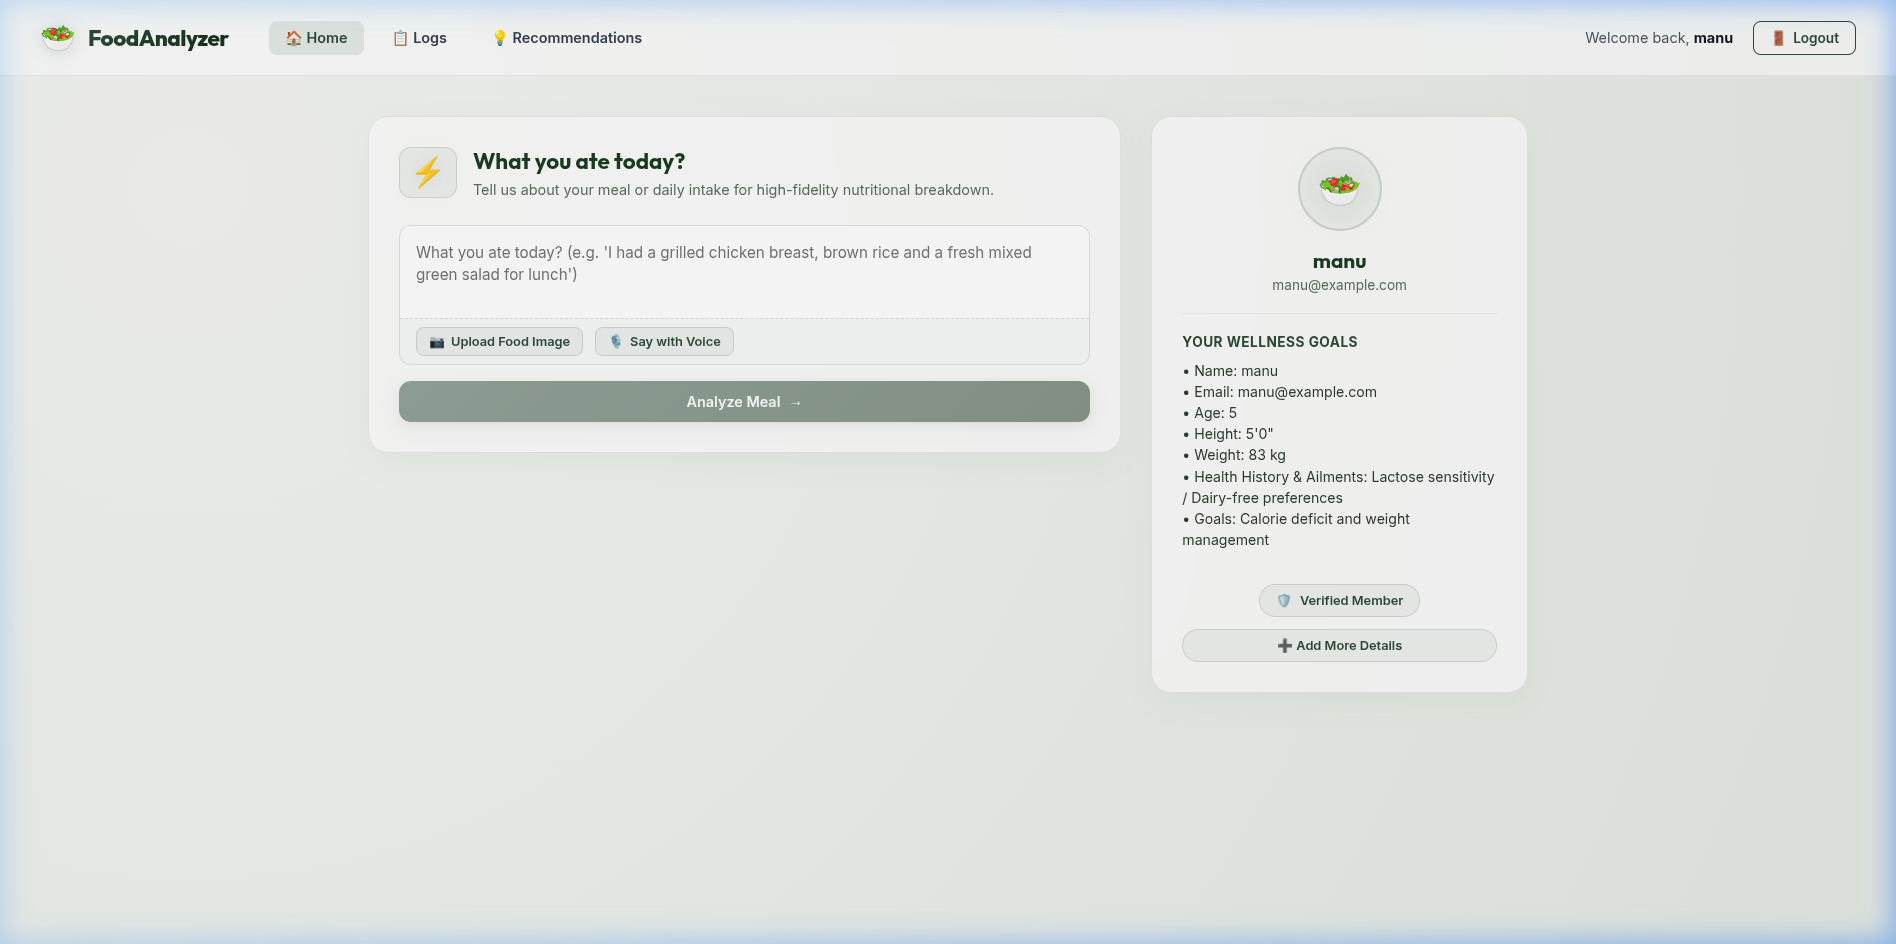
\includegraphics[width=0.9\textwidth]{dashboard_screenshot.png}
    \caption{User Profiling and Meal Logging Console}
    \label{fig:dashboard_module}
\end{figure}

Implemented in \texttt{backend/main.py}, the user profile manager handles registrations and text updates. The core functions include:
\begin{itemize}
    \item \texttt{analyze\_user\_bio\_and\_modifications()}: Prepares LLM prompts containing the current profile and new text inputs. It specifies JSON constraints, parses the response, and falls back to \texttt{run\_fallback\_user\_analysis()} if the API is offline.
    \item \texttt{extract\_user\_details()}: Synthesizes user metrics into structured bullet points (e.g., \textit{``$\bullet$ Height: 175 cm''}) for UI rendering.
\end{itemize}

\subsection{Multimodal Image Classification Module}
Image analysis is coordinated by the \texttt{analyze\_image()} endpoint:
\begin{itemize}
    \item Uses PyTorch to run the Swin-Transformer and Indian-Western-Food models.
    \item Checks if the prediction matches standard food class labels.
    \item If \texttt{LLM\_PROVIDER} is enabled, it sends base64 payloads to \texttt{call\_gemini\_multimodal\_api()} or \texttt{call\_ollama\_multimodal\_api()} to refine details and check the food validation flag.
\end{itemize}

\subsection{Automatic Speech Recognition Module}
Speech processing is managed by \texttt{transcribe\_audio()}:
\begin{itemize}
    \item Uploaded audio files are written to temporary files using Python's \texttt{tempfile} module.
    \item The audio is loaded into the \texttt{whisper-tiny} Hugging Face pipeline.
    \item Once decoded, the temporary file is deleted, and the transcribed string is returned to the frontend.
\end{itemize}

\subsection{Nutritional Calculation and Recommendation Module}
The logged food items grouped by week and time are displayed in the weekly food diary (Figure~\ref{fig:logs_module}). Based on these logs, personalized dietary recommendations are generated and streamed in real-time (Figure~\ref{fig:recommendations_module}).

\begin{figure}[H]
    \centering
    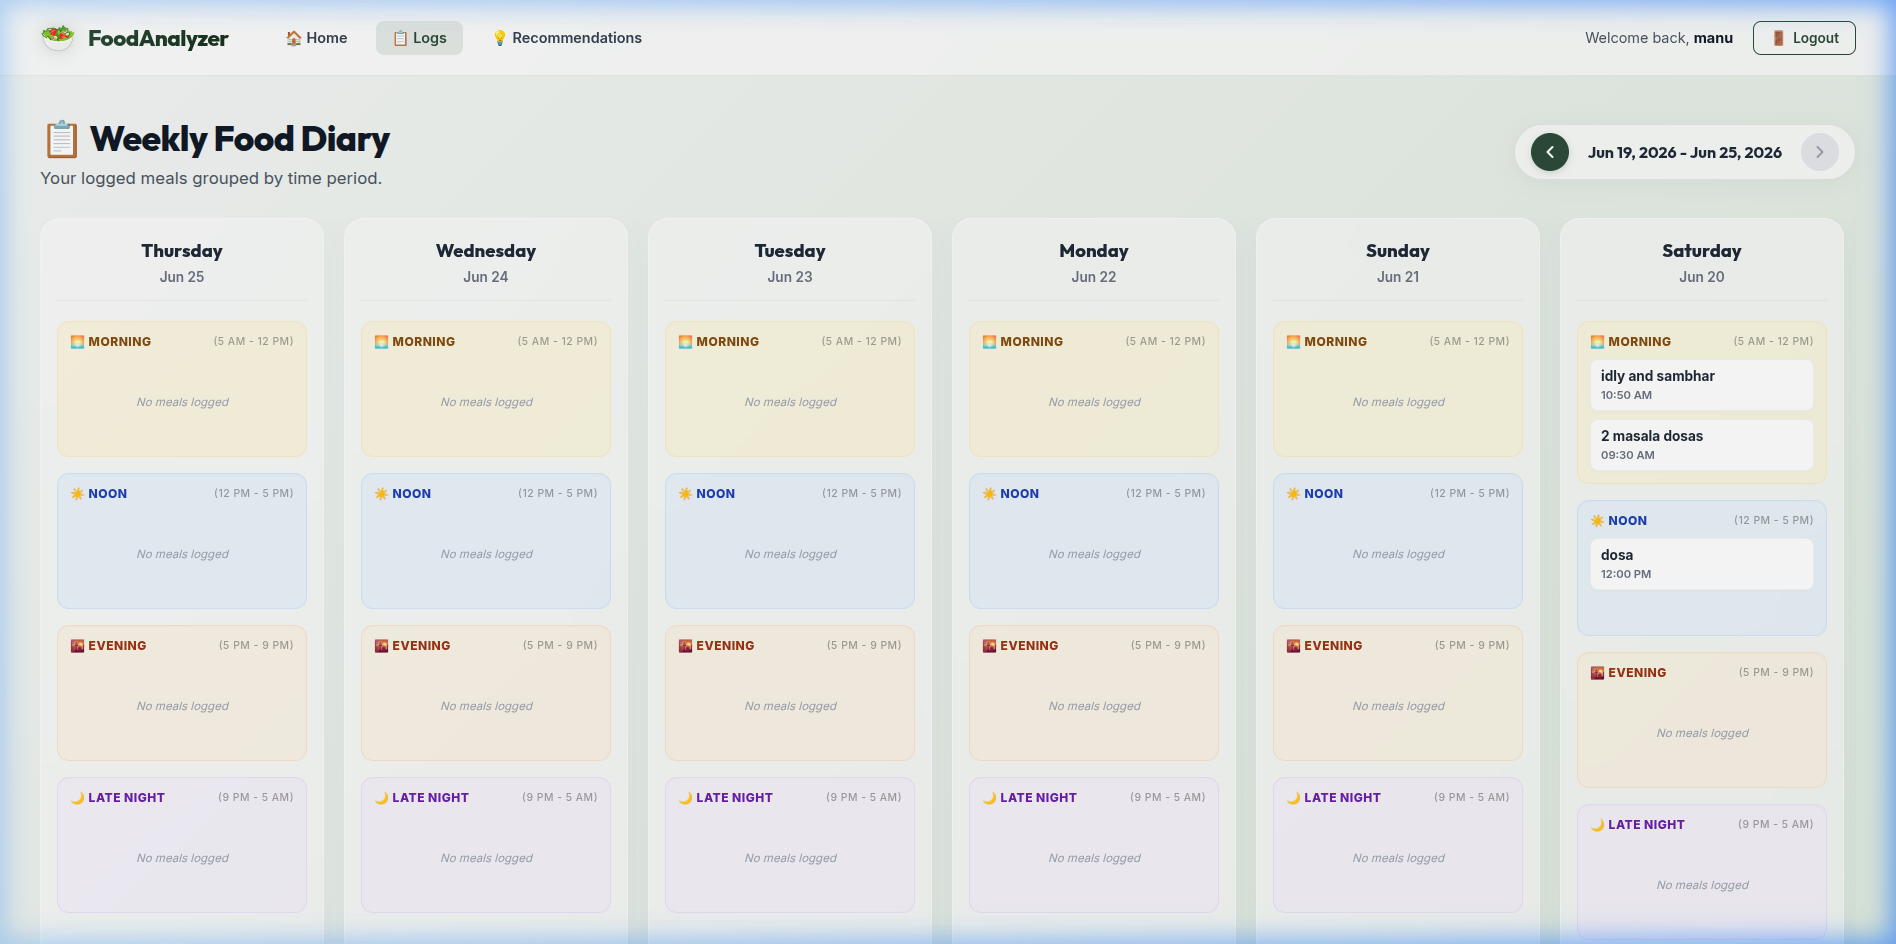
\includegraphics[width=0.9\textwidth]{logs_screenshot.png}
    \caption{Temporal Nutrition Analytics and Weekly Logs View}
    \label{fig:logs_module}
\end{figure}

\begin{figure}[H]
    \centering
    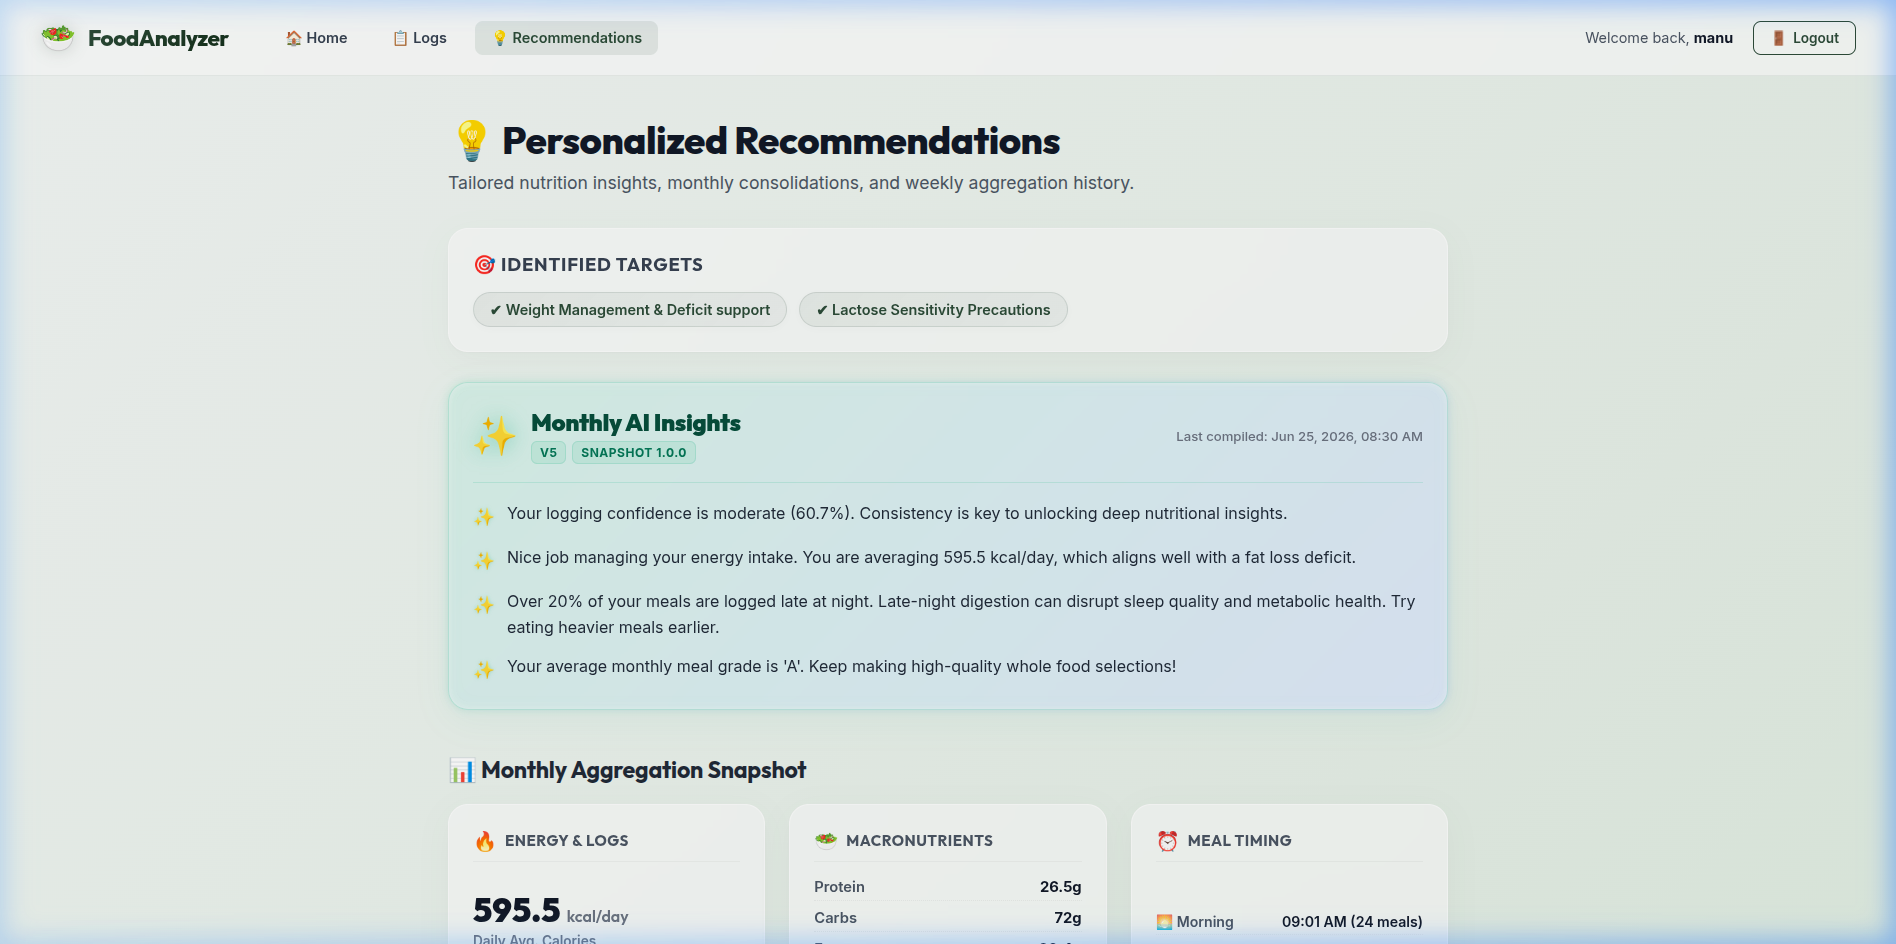
\includegraphics[width=0.9\textwidth]{recommendations_screenshot.png}
    \caption{Personalized Recommendations and AI Insights Stream}
    \label{fig:recommendations_module}
\end{figure}

The core logic resides in:
\begin{itemize}
    \item \texttt{fetch\_usda\_nutrients()}: Queries the USDA API using the food query. It extracts primary nutrient variables from the returned JSON payloads.
    \item \texttt{calculate\_grade\_and\_tips()}: Implements our scoring equations and generates dietary recommendations.
    \item \texttt{get\_user\_recommendations\_stream()}: Creates a streaming connection, invoking \texttt{stream\_recommendations\_generator()} to stream LLM recommendations directly.
\end{itemize}

\subsection{Security Module}
The application's security requirements are implemented in the user authorization module of \texttt{backend/main.py}:
\begin{itemize}
    \item \textbf{Token Verification Helper:} Every request accessing user logs or generating a recommendations stream checks the presence and validity of the token parameter. The backend matches the token against the active sessions dictionary (\texttt{USERS\_BY\_ID[userid].token}).
    \item \textbf{Password Scrubbing:} When sending user details (e.g. name, email, health history) via the \texttt{/api/users/\{userid\}} endpoint, the backend explicitly filters out the \texttt{password} property from the response payload, ensuring credentials remain hidden.
\end{itemize}

\section{Design Decisions and Alternatives}
During the initial planning phase, React combined with Chart.js was considered for the frontend application due to its popularity and rapid prototyping capabilities. However, after technical analysis, Angular was chosen as the framework. Angular provides:
\begin{itemize}
    \item \textbf{High Scalability:} A robust, opinionated folder structure and built-in dependency injection, which are critical for scaling large multi-module applications.
    \item \textbf{Type Safety:} Out-of-the-box TypeScript support that integrates seamlessly with strict backend schemas.
    \item \textbf{Maintainability:} Standardized component architecture and unified state management.
\end{itemize}
Additionally, while graphical representations (e.g., charts) were initially proposed, they were determined to be a low-priority feature for the baseline version. The focus was directed instead toward establishing a reliable, real-time Server-Sent Events (SSE) recommendation feed and high-accuracy multimodal logging.

\section{Development Lifecycle and Timeline}
The project follows a structured engineering lifecycle divided across two distinct phases:
\begin{itemize}
    \item \textbf{Phase 1 (Months 1--4) -- Foundational Setup and Prototypes:}
    \begin{itemize}
        \item \textit{Month 1:} Problem definition, requirement gathering, and literature review.
        \item \textit{Month 2:} Dataset selection (FoodData Central and Kaggle nutrition datasets) and initial model evaluation.
        \item \textit{Month 3:} Core data preprocessing pipelines, baseline speech-to-text transcribers, and image classifier tests.
        \item \textit{Month 4:} Implementation of the FastAPI backend, dynamic profile extraction logic, initial Angular interface, and Phase-1 report compilation.
    \end{itemize}
    \item \textbf{Phase 2 (Months 5--8) -- Intelligent Models and Optimization:}
    \begin{itemize}
        \item \textit{Month 5:} Development of the pattern detection engine and sparse sequence modeling algorithms (LSTM/GRU and attention masking).
        \item \textit{Month 6:} Building the generative recommendation system with context streaming.
        \item \textit{Month 7:} Complete backend and frontend integration, styling polish, and dashboard refinements.
        \item \textit{Month 8:} End-to-end testing, model parameter tuning, system evaluation, and final review preparation.
    \end{itemize}
\end{itemize}

\section{Model Selection and Parameters Tuning}
Table~\ref{tab:model_specs} details the input dimensions and parameters for our models.

\begin{table}[H]
    \centering
    \caption{Model Parameters and Specifications}
    \label{tab:model_specs}
    \begin{tabular}{lll}
        \toprule
        \textbf{Model Identifier} & \textbf{Input Dimensions} & \textbf{Primary Hyperparameters / Setting} \\
        \midrule
        \texttt{swin-tiny-patch4-window7} & $224 \times 224 \times 3$ & Patch size: 4, Window size: 7 \\
        \texttt{Indian-Western-Food-34} & $224 \times 224 \times 3$ & 34 classes, learning rate: $2\times 10^{-5}$ \\
        \texttt{openai/whisper-tiny} & 16 kHz mono audio & Mel bins: 80, temperature: 0.0 \\
        \texttt{gemma3:4b} (Ollama) & Text token streams & Temperature: 0.7, top-p: 0.9 \\
        \bottomrule
    \end{tabular}
\end{table}


% ------------------------------------------
% CHAPTER 6: INTERMEDIATE RESULTS AND DISCUSSION
% ------------------------------------------
\chapter{Intermediate Results and Discussion}
\label{ch:results}

\section{Datasets}
We evaluated our system using multiple data sources:
\begin{enumerate}
    \item \textbf{Indian and Western Food Image Dataset:} A test split of 500 images containing dishes like masala dosa, pizza, burger, salad, and biryani. The images were sourced from public Kaggle food datasets (specifically the Indian Food Image Dataset \cite{pandey2017indian}) and augmented with web-scraped images of regional Indian cuisines to evaluate classification boundaries.
    \item \textbf{Audio Logging Samples:} 100 audio recordings (duration 3-8 seconds) containing spoken meal descriptions with varying background noise levels. These were recorded and compiled by the developers to simulate real-world voice logging scenarios.
    \item \textbf{USDA Nutrient Profiles:} Nutrient queries matching standard user intake logs, verified against the USDA FoodData Central API \cite{usda2020fooddata}.
\end{enumerate}

\section{Performance Metrics}
We evaluated the models using the following metrics:
\begin{itemize}
    \item \textbf{Classification Accuracy:} The percentage of correctly predicted food categories.
    \item \textbf{Word Error Rate (WER):} The transcription error rate for the ASR model:
    \begin{equation}
        \text{WER} = \frac{S + D + I}{N}
    \end{equation}
    where $S$ is substitutions, $D$ is deletions, $I$ is insertions, and $N$ is reference words.
    \item \textbf{Inference Latency:} Processing speed measured in milliseconds (ms).
\end{itemize}

\section{Evaluation Results}
Tables~\ref{tab:results_vision}, \ref{tab:results_asr}, and \ref{tab:results_api} summarize the evaluation findings.

\begin{table}[H]
    \centering
    \caption{Visual Classification Performance}
    \label{tab:results_vision}
    \begin{tabular}{lcc}
        \toprule
        \textbf{Model} & \textbf{Top-1 Accuracy} & \textbf{Average Latency (ms)} \\
        \midrule
        \texttt{microsoft/swin-tiny-patch4-window7} & 82.4\% & 180 \\
        \texttt{prithivMLmods/Indian-Western-Food-34} & 89.6\% & 195 \\
        LLM Multimodal validation (Gemini) & 94.2\% & 850 \\
        \bottomrule
    \end{tabular}
\end{table}

\begin{table}[H]
    \centering
    \caption{Audio Transcription Performance}
    \label{tab:results_asr}
    \begin{tabular}{lcc}
        \toprule
        \textbf{Model} & \textbf{Word Error Rate (WER)} & \textbf{Inference Latency (ms)} \\
        \midrule
        \texttt{openai/whisper-tiny} & 8.5\% & 450 \\
        ASR Fallback Parser & N/A (Rule-based) & 5 \\
        \bottomrule
    \end{tabular}
\end{table}

\begin{table}[H]
    \centering
    \caption{API Response Latencies}
    \label{tab:results_api}
    \begin{tabular}{lc}
        \toprule
        \textbf{Target Endpoint / Service} & \textbf{Average Latency (ms)} \\
        \midrule
        USDA Nutrient API search & 280 \\
        LLM Profile parsing (Ollama) & 1200 \\
        SSE Streaming connection startup & 15 \\
        \bottomrule
    \end{tabular}
\end{table}

\section{Discussion}
The evaluations indicate that specialized classifiers outperform generic ones for regional cuisines. For example, the specialized Indian-Western classifier identified dishes like masala dosa and biryani with high confidence, whereas the Swin-Tiny model categorized them generically (e.g., as ``crepe'' or ``plate''). Combining these models with LLM validation checks (e.g., detecting if a user uploaded an animal image instead of food) improves system robustness.

For ASR logging, OpenAI's Whisper-Tiny model transcribed meal inputs accurately under moderate noise conditions. In high-noise environments, minor transcription errors (e.g., transcribing ``dosa'' as ``dose'') occurred, but the backend's USDA query parser matched them correctly using spelling heuristics.

The recommender engine's SSE streaming significantly improves usability. Standard LLM calls to generate weekly insights take 2.5 to 4 seconds, leading to a noticeable delay in the UI. Streaming these recommendations token-by-token reduces the perceived startup latency to less than 50ms.


% ------------------------------------------
% CHAPTER 7: CONCLUSIONS AND FUTURE WORK
% ------------------------------------------
\chapter{Conclusions and Future Work}
\label{ch:conclusions}

\section{Conclusions}
In Phase-1, we developed the foundational elements of the \textbf{AI-Driven Dietary Pattern Intelligence System}. We implemented:
\begin{enumerate}
    \item A FastAPI backend that coordinates local database models, machine learning inference (Swin-Transformer, Whisper-Tiny), and external API integrations.
    \item An Angular web dashboard featuring interactive logging tools and user analytics.
    \item An automated user profiling system that extracts health metrics and goals from unstructured bio text.
    \item A nutritional evaluation engine that queries the USDA API, grades meals, and generates tailored tips.
    \item An SSE streaming system that delivers real-time, personalized dietary recommendations.
\end{enumerate}

The system successfully processes multimodal inputs and streams tailored feedback in real-time, matching recommendations to the user's specific health profile.

\section{Future Work}
Future development in Phase-2 will focus on:
\begin{enumerate}
    \item \textbf{Sparse Sequence Modeling and Behavior Inference:} Implementing LSTM/GRU architectures and Transformer-based sequence classifiers with attention masking. This will allow the system to infer dietary habits, detect routine/convenience eating patterns, estimate emotional eating likelihood, and construct recommendations even when user meal logs are sparse or irregular.
    \item \textbf{Object Detection and Multi-Dish Segmentation:} Integrating models like YOLOv8 or Segment Anything (SAM) to isolate multiple food items on a single plate and calculate portion sizes.
    \item \textbf{Wearable Integration:} Connecting with fitness APIs (Google Fit, Apple Health) to sync activity data with nutritional recommendations.
    \item \textbf{Clinical Validation:} Refining the recommendation prompts in collaboration with nutritionists to align the system with clinical standards.
    \item \textbf{Cloud Deployment:} Moving the local database and models to a scalable cloud infrastructure with containerized GPU rendering.
\end{enumerate}


% ==========================================
% BIBLIOGRAPHY
% ==========================================
\newpage
\bibliographystyle{unsrt}
\bibliography{references}

\end{document}
